\documentclass{standalone}
\usepackage{tikz}
\usetikzlibrary{positioning,fit,matrix}
\usepackage{todonotes}
%\usepackage{scalefnt}

%\tikzset{%
%  textnode/.style     = {\sffamily font=\fontsize{10}{12.4}\selectfont},
%}

\begin{document}

\sffamily%\sansmath
%\scalefont{0.01}
%\fontsize{8}{10.0}\selectfont

\begin{tikzpicture}





% L2
\node[inner sep=0] (alex1) {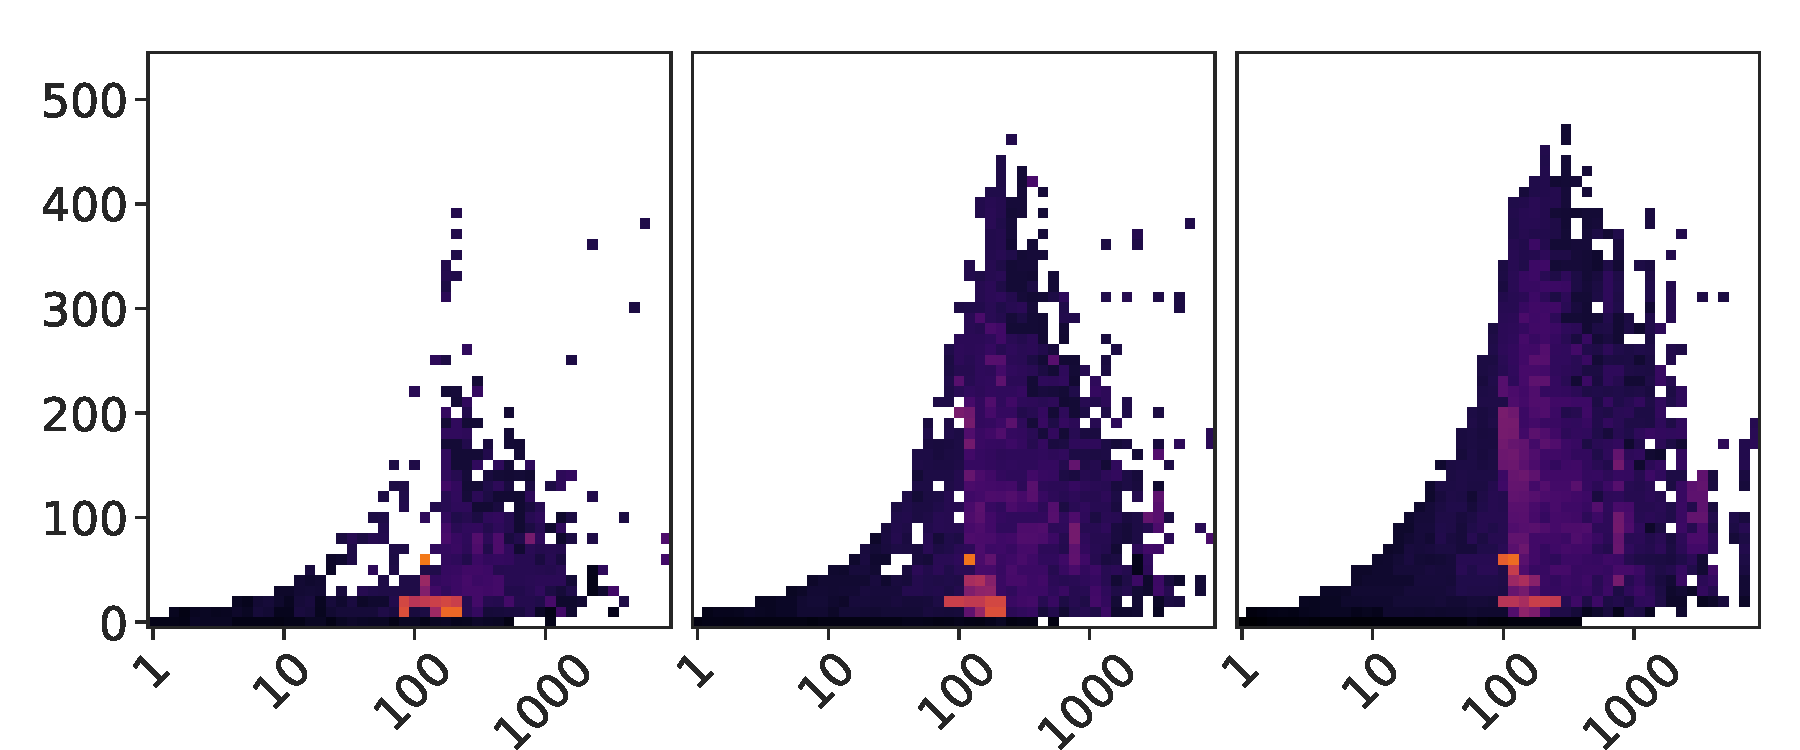
\includegraphics[width=6cm]{alex1.pdf}};


% CBar
%\node[inner sep=0, below=0mm of alex1] (cbar1) {\includegraphics[width=6cm]{plots/peppercorn-cbar-meanStruct.pdf}};
\node[inner sep=0, right=0mm of alex1,rotate=90,anchor=north,align=center,shift={(0.0,0.0)}] (cbar1) {
\includegraphics[width=3.5cm]{cbar1.pdf}};
\node[color=black,right=1mm of cbar1,rotate=90,anchor=north,align=center,shift={(-1.70,0.0)}] {Mean struct. size};


% Titles
%\node[color=black,above=5mm of alex1,rotate=0,anchor=north,align=center,shift={(0.20,0.00)}] {Mean Struct. Size};
\node[color=black,below=0mm of alex1,rotate=0,anchor=north,align=center,shift={(0.20,0.00)}] {Nr. of reactions};
\node[color=black,left=3mm of alex1,rotate=90,anchor=north,align=center,shift={(0.0,0.0)}] {Nr. of struct.};

\node[color=black,above=1.5mm of alex1,rotate=0,anchor=north,align=center,shift={(-1.60,0.00)}] {\tiny{$k=(2,3)$}};
\node[color=black,above=1.5mm of alex1,rotate=0,anchor=north,align=center,shift={(0.20,0.00)}] {\tiny{$k=(4,5)$}};
\node[color=black,above=1.5mm of alex1,rotate=0,anchor=north,align=center,shift={(2.00,0.00)}] {\tiny{$k=(6,7)$}};


%\node[color=black,left=3mm of baseline1,rotate=90,anchor=north,align=center,shift={(0.0,0.0)}] {\textbf{L1}};
%\node[color=black,left=3mm of alex1,rotate=90,anchor=north,align=center,shift={(0.0,0.0)}] {\textbf{L2}};
%\node[color=black,left=3mm of tetra1,rotate=90,anchor=north,align=center,shift={(0.0,0.0)}] {\textbf{L3}};


\end{tikzpicture}

\end{document}
